\documentclass[final]{siamltexmm}

\usepackage{graphicx}
\usepackage{algorithm}
\usepackage{algorithmic}
\newcommand{\pe}{\psi}
\def\d{\delta} 
\def\ds{\displaystyle} 
\def\e{{\epsilon}} 
\def\eb{\bar{\eta}}  
\def\enorm#1{\|#1\|_2} 
\def\Fp{F^\prime}  
\def\fishpack{{FISHPACK}} 
\def\fortran{{FORTRAN}} 
\def\gmres{{GMRES}} 
\def\gmresm{{\rm GMRES($m$)}} 
\def\Kc{{\cal K}} 
\def\norm#1{\|#1\|} 
\def\wb{{\bar w}} 
\def\zb{{\bar z}} 

% some definitions of bold math italics to make typing easier.
% They are used in the corollary.

\def\bfE{\mbox{\boldmath$E$}}
\def\bfG{\mbox{\boldmath$G$}}

\title{Music Genre Classification}
\author{Hung-Ting Wen\thanks{\tt htw230@nyu.edu}
        \and Yun-shao Sung\thanks{\tt yss265@nyu.edu}}

\begin{document}
\maketitle

\begin{abstract}
Our purpose of this project is to build a learning machine that can distinguish between different music genres.  We will implement and experiement on several proposed methods to music genre classification and see if we can achive, or even outperform, results from researches.  Our baseline would be 2nd-order coefficients combined with SVM classifier.  After then, we will move on to Sparse Representation Classifier.
\end{abstract}

\pagestyle{myheadings}
\thispagestyle{plain}

\section{Introduction}
Classifying music genre has never been an easy task, even for human beings.  Modern music has its own family tree, and certain features of an ancester will be inherited by its decendents and that make classification sometimes impossible.  However, for some music applications that constantly recommend musics to its users, a good classification is their basics to recommendation system.

\section{Performance Criterion}
For each run, we will randomly split 90\% of the samples as training set and the remaining 10\% as the test set. The performance criterion will based on 1) the length of texture window, 2) analysis window, and the classification accuracy of averaged result over 10 trails.

\begin{figure}[ht]
\begin{center}
  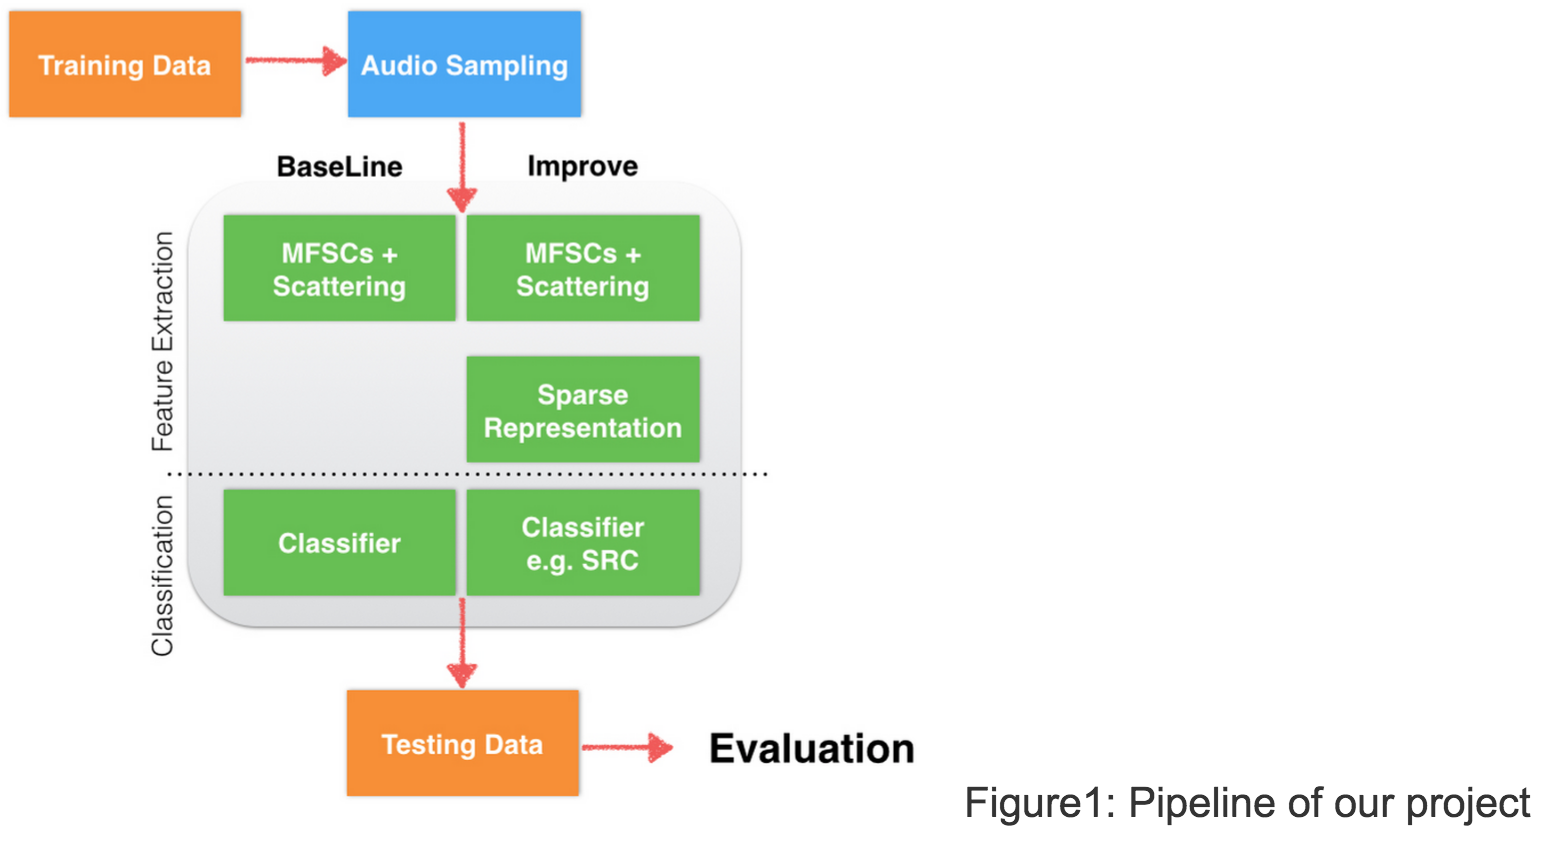
\includegraphics[scale=0.3]{Figure1.png}
\end{center}
\end{figure}

\section{Background}
To have the mel-frequency spectral coefficients (MFSC), we need to relate them to wavelet transform. The Fourier Transform of x(t) is:
\begin{equation}
X(w)=\int x(u)e^{(-iwu)}du\label{eq1}
\end{equation}
And if we frame the signal into short frame which xt,T(u) = x(u)wT(u-t), where wT is time frame window of size T:
\begin{equation}
X_{t,T}(w)=\int x_{t,T}(u)e^(-iwu)du\label{eq2}
\end{equation}
MFSCs are obained by averaging the spectrogram $\arrowvert X_{t,T}(w)\arrowvert^{2}$ over me-frequency interval, which these intervals have constant frequency for bandwidth below 1000Hz and above 1000Hz. Then MFSCs can be written as:
\begin{equation}
M_{T}x(t,j)=\frac{1}{2\pi} \int \arrowvert X_{t,T}(w)\arrowvert^{2} \arrowvert \widehat{\Psi}_{j}(w) \arrowvert^{2} dw\label{eq3}
\end{equation}
where $\widehat{\Psi}_{j}(w)$ covers a me-frequency interval that indexed j.

With Parseval’s and Convolution theorem  applied:
\begin{equation}
M_{\lambda}x(t,j)=\int \arrowvert x_{t,T} \star \Psi_{j}(u) \arrowvert^{2} du\label{eq4}
\end{equation}
where $\Psi_{j}$ can be interpreted as dilations of a mother wavelet $\Psi for \lambda > \lambda_{0}$, and this formula gives us the energy of x in a neighborhood of t of size T and in the mel-frequency interval indexed by j. Due to it’s properity that not able to capture the non-stationary structures of duration shorter than T, we may need choose the T to be small, and previous paper used 23ms.
  
Then we can use $\{ \Psi_{\lambda}\}_{\lambda \in \Lambda}$ as our wavelet filter bank, and then the resulting wavelet transform defined by:
\begin{equation}
W_{x}(t)=\left( \begin{array}{cc}
x \star \phi(t) \\
x \star \Psi_{\lambda}(t)
\end{array} \right)_{\lambda \in \Lambda}\label{eq5}
\end{equation}
where $\phi$ is a low-pass filter covering the low-frequency interval not covered our wavelet filters.

\section{Application}
For the collection of mel-frequency bank, we will use the tool from ScatNet to generate a series mel-frequency looks like Figure4.1.  The frequency generator our reference paper used is the Galbor filer:
\begin{equation}
\Psi(t)=\theta(t)e^{i2\pi Qt} \Rightarrow \Psi(t)=\theta(t)\cos(2\pi Qt) + \theta(t)\sin(2\pi Qt)\label{eq6}
\end{equation}
where $\theta$ is Gaussian, with $Q=16$ and $P=23$.  We think the idea for the series of frequency is that they need to have certain overlap. Therefore, when we are doing scaltering cascade for the filter $\lambda_{i} \dots \lambda_{n}$,  the signal not being filtered, or emphasized by $\lambda_{i}$ will be captured and emphasized by $\lambda_{i+1} \dots \lambda_{n}$, which are the neighbor filters. We may also insterested to check the effect of the frequency collections to the classfication accuracy, although larger frequency collection implies larger feature vector, which will increase complutation times.
\begin{figure}[ht]
\begin{center}
  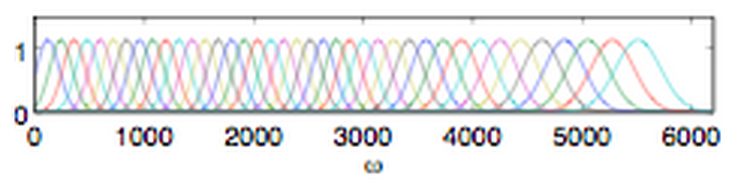
\includegraphics[scale=0.8]{Figure2.png}
  \caption{Collection of mel-frequency}
\end{center}
\end{figure}
For the mel-frequency scattering part, we will use (\ref{eq5}), which it will output the low-passed signal $x \star \phi_{J}$, and, at next layer, each $\arrowvert x \star \Psi_{j_{1}} \arrowvert$ is again retransformed by (\ref{eq5}), which outout $\arrowvert x \star \Psi_{j_{1}} \arrowvert \star \phi_{J}$ and then computes $\arrowvert \arrowvert x \star \Psi_{j_{1}} \arrowvert \star \Psi_{j_{2}} \arrowvert \star \phi_{J}$ in the next layer(Figure4.2).
\begin{figure}[ht]
\begin{center}
  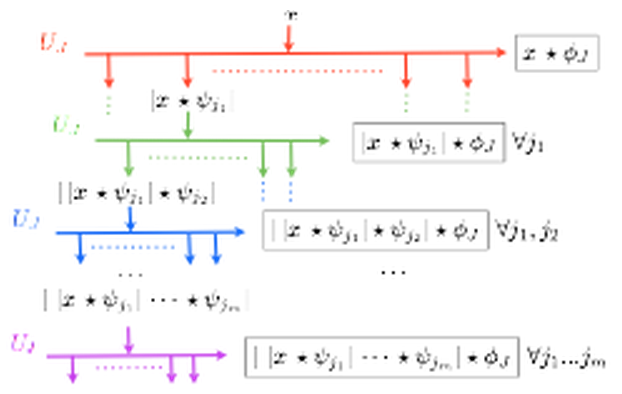
\includegraphics[scale=0.5]{Figure3.png}
  \caption{Scattering cascade}
\end{center}
\end{figure}

\section{Baseline}
Our baseline will be using 2nd-order Scattering Coefficients for feature extraction.  Combining with SVM classifier, we are expecting to achieve roughly about 85\% accuracy as indicated in the paper.
\begin{algorithm}[htb]
  \caption{2nd-order Scattering Coefficients}
  \label{algo:SC}
\begin{algorithmic}[1]
  \FOR{$x \in X$}
    \FOR{$t=1 \dots T$}
      \STATE OUTPUT $x \star \phi(t)$
      \STATE
        \FOR{$\lambda_{1} \in \Lambda$}
          \STATE OUTPUT $\arrowvert x \star \Psi_{\lambda_{1}} \arrowvert \star \phi(t)$
          \STATE COMPUTE $x \star \Psi_{\lambda_{1}}$
          \STATE
            \FOR{$\lambda_{2} \forall \lambda_{2} \in \Lambda s.t. \lambda_{2} > \lambda_{1}$}
              OUTPUT $\arrowvert \arrowvert x \star \Psi_{\lambda_{1}} \arrowvert \star \Psi_{\lambda_{2}} \arrowvert \star \phi(t)$
            \ENDFOR
        \ENDFOR
    \ENDFOR
  \ENDFOR
\end{algorithmic}
\end{algorithm}

We will use Numpy for implementation.  Numpy provides convolve, flatten, and other functions that can help us build our own implementation.

\section{Problem formulation of further improvement}
This is the part for the further improvement after baseline method. We will combine the scalled feature vector followed by transforming into sparse representation, which governed by the formula below:
\begin{equation}
(l^{l}): argmin_{\omega \in \Re^{p}} \frac{1}{2} \arrowvert x - D_{\omega} \arrowvert_{2}^{2} + \lambda \arrowvert \omega \arrowvert_{1}\label{eq7}
\end{equation}
where $D$ is a $N$ by $P$ dictionary matrix, and $\omega$ is a $P$ by $M$ matrix. The size of column which is $P$ in dictionary is the length of atoms or codewords, and the purpose of dictionary is to sparsifies the representation such that can fit $\arrowvert \omega \arrowvert_{0}^{0} < L$, where $L$ is the number of non-zero element of each column of $omega$.  In (\ref{eq7}), we are both learning $D$ and $\omega$ from data $x$, and the goal is to have the final $\omega$ sparse representation so each of x can have it’s own sparse representation, and then perform classification base on the representation.

(\ref{eq7}) will yield the following interesting questions: \\
1. How we decide the size of atoms? In other word, how should we decide dictionary’s number of colums. One approach will be just copy xT, which means number of atoms equals to number of data samples. However, we think this huge dictionary will be very costly during optimization. The alternative might be the number of top best principal component analsis (PCA). If we can get the top best P number of PCA axises, then it may means there are P components existed that can seperate x into clear differernt groups. \\
2. What’s the strategy of optimizating (\ref{eq7}), after dictionary initialized in previous step? The first setp will be spase coding, which we can perform by Relaxation (or Baisis Pursuit) or Greedy approaches. For Relaxation approach, the newly defined function will be convex, and there are plenty of algorithm for sovling this like Interior Point Method and Iterative shrinkage. As for Greedy approach, Matching Pursuite can be the method to apply. \\

Then, the next step will be dictionary update. Based on K-SVD method, we can randomly select the atom in dictionary and find out all the signal that use the atom and we like to very optimize the current selected atom by substracting the contributions of every other atom. Repeat this atom updating for all atom in dictionay then we are done with dictionay and we can repeat sparse coding and so on until the error converge or hit the prefix number of iteration.

\begin{figure}[ht]
\begin{center}
  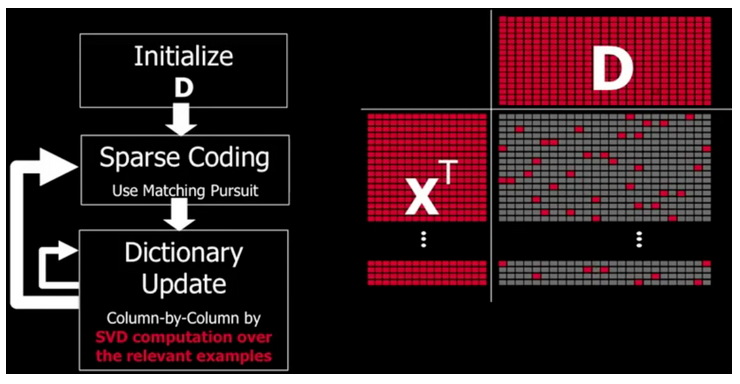
\includegraphics[scale=0.8]{Figure4.png}
  \caption{K-SVD Algorithm}
\end{center}
\end{figure}

\section{Algorithm used in reference paper} \\
The algorithm being used in reference paper are the combinations of scattering of mel-frequency cepstral coefficients (MFCCs), and sparse representation followed by sparse representation classifier (SRC). As for the baseline method, we will only use 2nd-ordered scattering method alone with classification (e.g. SVM) to see the performance and accuracy. The accuracy for this method that listed in the reference is about 82\% under 1.5s texture window(Figure7.1), and our gaol for this baseline method will be trying to reproduce the accuracy. Further, we will also be interested to test the accuracy if we expand the scattering to 3rd-order.

For our further improvement, we will like to do the combination of scattering plus transformation to sparse transformation. The idea of the scattering method is that it reduce the in-class variability of signals while still preserving the most of the signal energy. According to the author, 1st-ordered scattering is good enough, and higher orders provide complementary information.  Then, the idea of transforming feature vector to spase representation is a data-driven approach, andit will find high dimention and yet sparse encoding of each example with respect to the dictionary. Although some concerns may rise regarding to the enlarging dictionary for better classification performance may decrease the performance, the author claimed dictionary will learn from scattering coefficients to represent the residual in-class variability of the vectors of scattering coefficients. This implies transforming dense high-dimentional scattering representation into a sparse representation by this relative small dictionary could work well together, and is the main issue we set to dicover. Our expected accuracy for this approach will be 89.8\%(Figure7.2).

\begin{figure}[ht]
\begin{center}
  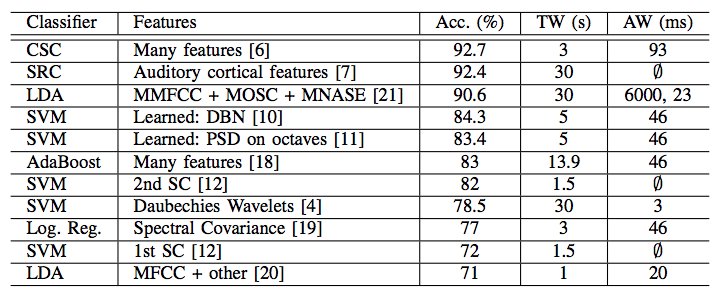
\includegraphics[scale=0.8]{Figure5.png}
  \caption{Genre recognition accuracy of various algorithm on  GTZAN dataset}
  \label{fig5}
\end{center}
\end{figure}

\begin{figure}[ht]
\begin{center}
  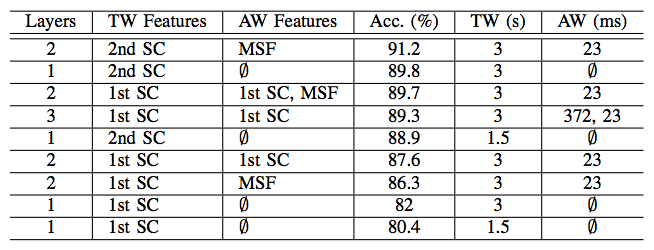
\includegraphics[scale=0.8]{Figure6.png}
  \caption{Genre recognition accuracy of proposed method on  GTZAN dataset (using SRC)}
  \label{fig6}
\end{center}
\end{figure}

\section{Datasets}
To make comparable results, we will use the same data set as the paper used: GTZAN.  This dataset consists of 1000 audio clips, each 30sec long.  The dataset contains 10 genres, each of whom has 100 tracks.  Each track is 22050Hz mono 16-bit file in .wav format.

\begin{thebibliography}{10}
\bibitem{fpf} {\sc Low pass filter by FFT convolution}, {\em http://www.dsprelated.com/freebooks/sasp/Example\_1\_Low\_Pass\_Filtering.html}
\bibitem{msc} {\sc Multiscale Scattering for Audio Classifications}, {\em http://www.cmap.polytechnique.fr/scattering/ismir-final.pdf}
\bibitem{dl} {\sc Digital image processing: p067- Dictionary Learning}, {\em https://www.youtube.com/watch?v=XLXSVLKZE7U}
\bibitem{ipm} {\sc Interior-point methods}, {\em https://web.stanford.edu/class/ee364a/lectures/barrier.pdf}
\bibitem{ista} {\sc Iterative Shrinkage/Thresholding Algorithms}, {\em http://people.ee.duke.edu/~lcarin/figueiredo.pdf}
\bibitem{mpwtfd} {\sc Matching pursuits with time-frequency dictionaries}, {\em http://www.cmap.polytechnique.fr/~mallat/papiers/MallatPursuit93.pdf}
\bibitem{eik} {\sc Efficient Implementation of the K-SVD Algorithm using Batch Orthogonal Matching Pursuit}, {\em http://www.cs.technion.ac.il/~ronrubin/Publications/KSVD-OMP-v2.pdf}
\end{thebibliography}

\end{document}
